\chapter{Arquitetura física}

Os componentes físicos do sistema estão enumerados abaixo:

\begin{itemize}
	\item $<<$HW$>>$ UART
	\item $<<$SW$>>$ Driver UART
	\item $<<$SW$>>$ ISR UART
	\item $<<$SW$>>$ Buffer UART
	\item $<<$SW$>>$ Controlador do elevador
	\item $<<$SW$>>$ Protocolo de comunicação
\end{itemize}

A interação entre estes componentes no sistema é apresentada na Figura \ref{fig:arq_fisica}.

\begin{figure}[h]
    \centering
    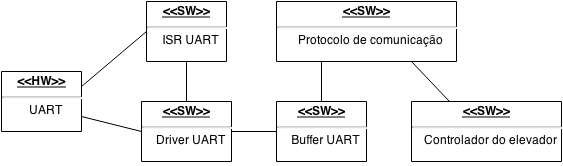
\includegraphics[width=0.8\columnwidth]{./figures/arq_fisica.png}
    \caption{Diagrama de blocos da arquitetura física do sistema.}
    \label{fig:arq_fisica}
\end{figure}

